\subsection{Application Context}

\subsection{System Profile}

\subsection{System Tasks}

\subsection{Dialog Structure}

\subsection{Mockups}

Upon starting the app on a capable device, the app presents itself as shown in Figure \ref{fig:start_mockup}.
This is effectively the start screen from where all the interaction takes place.
The green light in the top left shows that the app is detecting the marker with a high confidence, meaning that there are no large uncertainties.
If the marker is too warped or partially covered, the light switches to red.
If the app can still detect the marker but is having difficulties, the light switches to orange.
This mechanism is meant to offer fast and accurate feedback to the detection capability.
Another method of direct feedback is the already displayed axis-object.
This is meant to offer fast feedback to the orientation and scaling of the coordinate space to the user before a custom object is displayed.
The visibility of the axis-object can be toggled in the settings.

The menu button on the status bar at the bottom of the screen opens up a menu as seen in Figure ???.
From here the user can control the overlays they wish displayed over the camera view and control what is rendered into the picture.

\begin{figure}
	\centering
	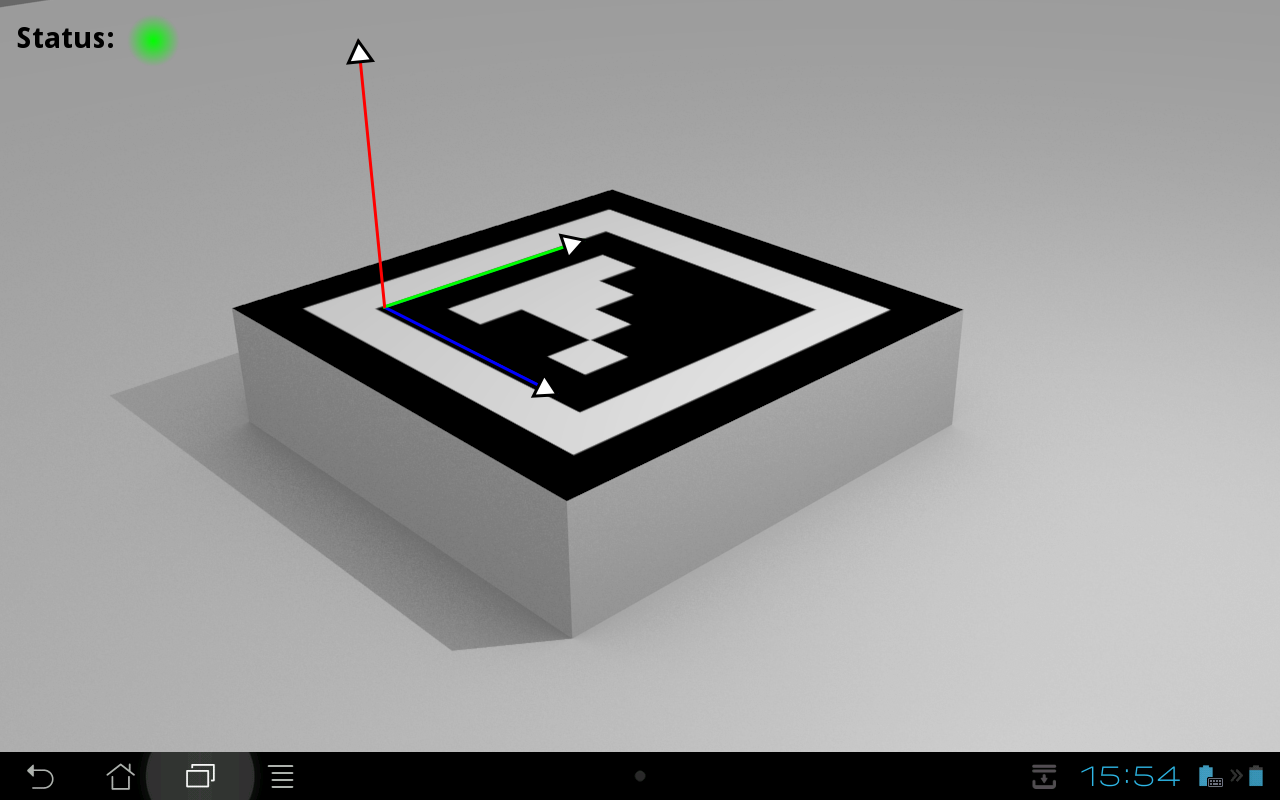
\includegraphics[width=15cm]{images/start_mockup.png}
	\caption[Start screen mockup.]{Mockup of how the start screen of the final app might look. Note the menu button on the bottom, the rendered axes, and the green status light signifying that the marker is being read with a high confidence.}
	\label{fig:start_mockup}
\end{figure}
